
\documentclass{article}
\usepackage[utf8]{inputenc}
\usepackage[bulgarian]{babel}

\usepackage{systeme}
\usepackage{amsmath}

\usepackage{cmap}
\usepackage[utf8]{inputenc}
\usepackage[T2A]{fontenc}

\newtheorem{definition}{Дефиниция}

\usepackage{comment}
%\use
\newtheorem{problem}{Задача}
\newtheorem{theorem}{Теорема}
\newcounter{solution}

\usepackage{graphicx}
\usepackage{pst-plot}

\usepackage{tikz}

\newcommand\solution{%
	\stepcounter{solution}%
	\textbf{Решение :}\\%
}

\usetikzlibrary{angles,
	quotes}
\usepackage{siunitx}


\date{}

\title{Книжка за упражнителни задачки на Деспина}
\begin{document}
	
	
	\maketitle
	\tableofcontents
	
	\section{Теория}
	
	\subsection{Триъгълник}
	
	
	\begin{tikzpicture}
	\draw
	  (0,0) coordinate[label=below:$A$] (a) --
	(4,0) coordinate[label=below:$C$] (c) --
	(4,4) coordinate[label=above:$B$] (b) -- cycle;
	
	
	\end{tikzpicture}
	

	
F=\tikz[scale=.625,baseline=0pt]{
	\clip[preaction=draw] (-30:1) -- (90:1) -- (210:1) -- cycle;
	\draw\foreach \i [count=\j] in {90,210,-30}{ 
		(\i:1) circle [radius=.25] (\i:.875) node [anchor=\i,font=\tiny] {\j}};}
	
	
	
	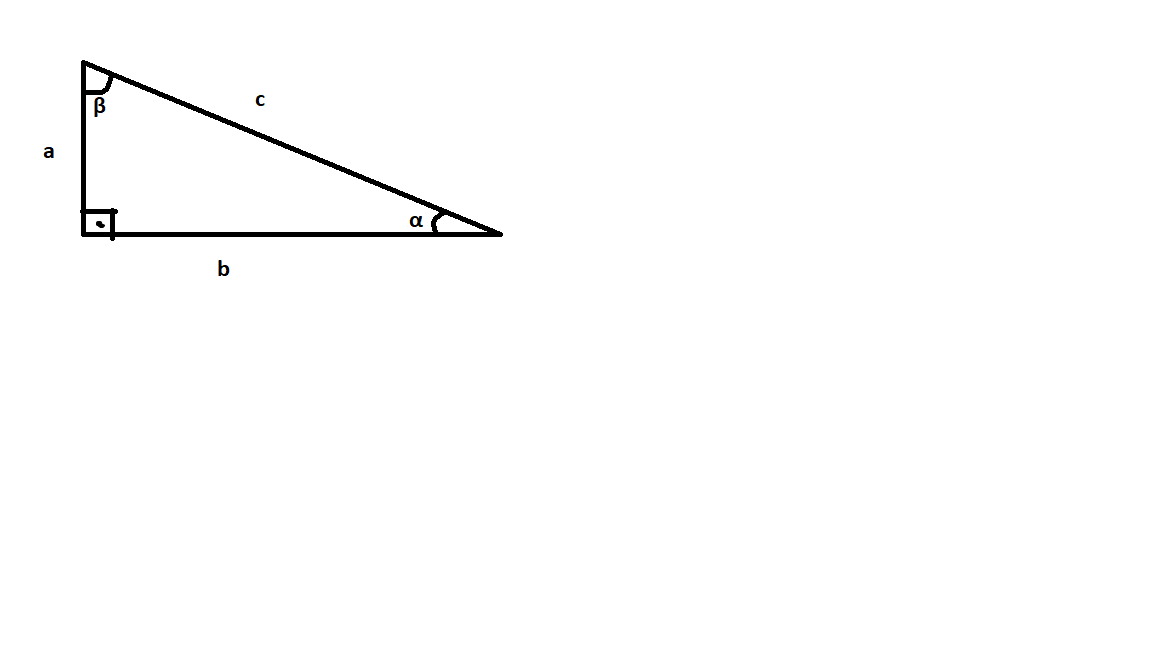
\includegraphics{Trig1}
	
	\vspace{-8cm}
	
	\begin{definition}$ sin(\alpha) = \frac{a}{c} $, $ cos(\alpha) = \frac{b}{c} $, $tg(\alpha) = \frac{a}{b} $, $cotg(\alpha) = \frac{b}{a} $	
	\end{definition}
Да зебележим, че $ sin(\beta) = cos(\alpha) = \frac{b}{c} $ и аналогично $cos(\beta) = sin(\alpha ) = \frac{a}{c} $.
$a^2 + b^2 = c^2  \to (\frac{a}{c})^2 + (\frac{b}{c})^2 = 1 \to sin^2(\alpha) + cos^2(\alpha) = 1$. \\
Тригонометрични тъждества ($\alpha, \beta \in [0,90] )$: \\
$sin^2(\alpha) + cos^2(\alpha) = 1$ \\
$ sin(\alpha) = cos(\beta) = cos(90 - \alpha) $ \\
$ tg(\alpha)cotg(\alpha) = 1 $ \\
$ tg(\alpha) = \frac{a}{b} = \frac{a}{c} \cdot \frac{c}{b} = \frac{sin(\alpha)}{cos(\alpha)} $, $cotg(\alpha) = \frac{1}{tg(\alpha)} = \frac{cos(\alpha)}{sin(\alpha)} $ 


\vspace{-6cm}

\subsection{Трапец}

	
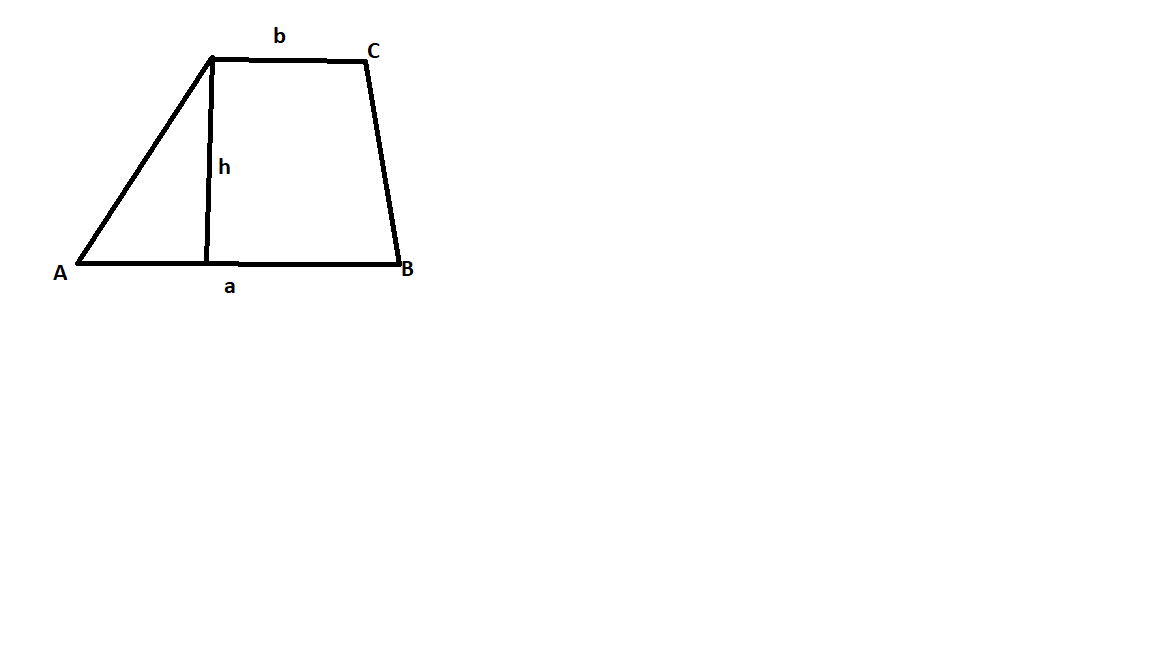
\includegraphics{Trapezoid}
\vspace{-8cm}

Лице на трапец: $S = \frac{a+b}{2}h$\\
Трапец, вписан в окръжност е равнобедрен.\\
Трапец описан около oкръжност: $AB + CD + AD + BC $, или сборът
на срещуположнисте страни е равен.


\subsection{Успоредник}


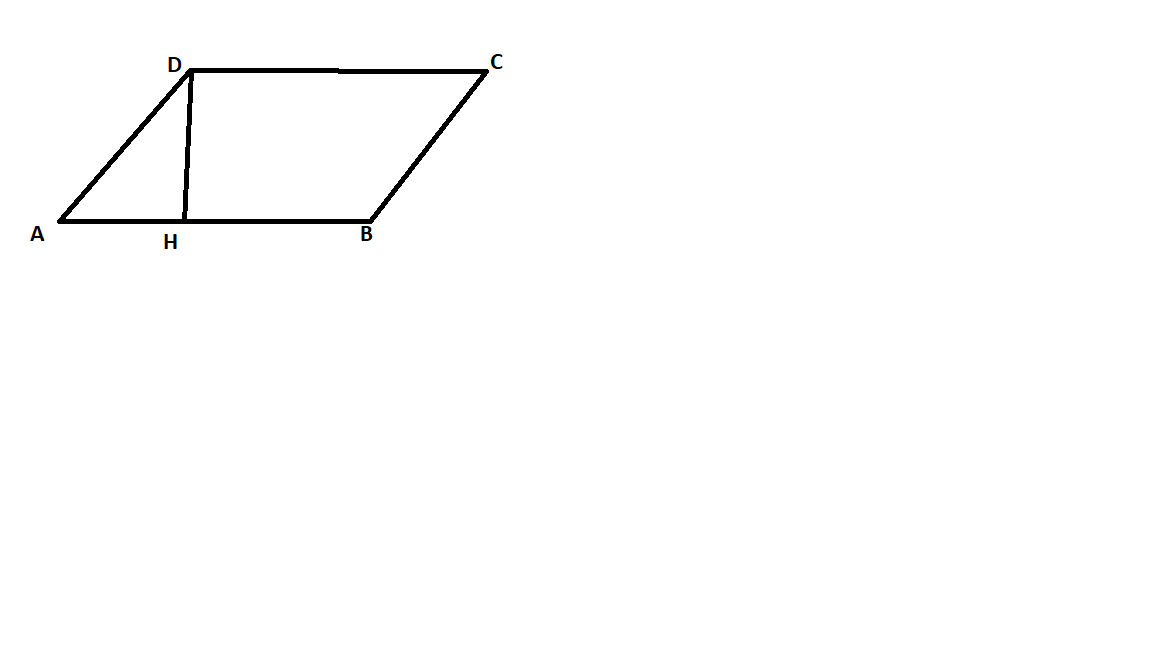
\includegraphics{Parallelogram}
\vspace{-6cm}

Страните са две по две успоредни $AB || CD$, $BC||AD $. 
Лице на успоредник: $S = AB \cdot DH$ (тук се разбира дължините на страните)

Коментари: $\triangle ABD \equiv \triangle  BCD $, 
 $\triangle ABC \equiv \triangle CDA $ \\
 $\angle BAD = \angle BCD $ и $ \angle ADC = \angle ABC $. $\angle ABC + \angle BAD = 180$.


Задачи - дадени са две страни на успоредник и ъгъл.

\subsection{Функции}
Функция е правило за съпоставяне на число по някакво правило. По-конкретно, имаме $x$, и на него съпоставяме $f(x)$.
Често се записва като $ y = f(x) $. Всичките $x$-ове, на които можем да съпоставим $f(x)$, се нарича дефиниционно множество на функцията $f(x)$. Графично се изобразяват наредените двойки $(x, f(x)) $ или $(x,y)$ в координатна система, в която по хоризонталата е стойността на $x$, a по вертикалата - на $y$.\\
Пример за фунцкия. $y =f(x) = x$.
Графиката минава през всички точки $(x,x)$ за $x$ в дефиниционното множество. Дефиниционното множество е цялата реална права. \\
Примери за функции, където деф. множество не е цялата права.
$y = \frac{1}{x}$(ДМ: $x \neq 0 $) и $y = \sqrt x$ (ДМ: $x \geq 0$)

\subsection{Линейна фунцкия}
$ y = f(x) = ax + b$ \\
Значеения на буквите a,b,c:
а - "колко стръмна е правата" \\
a>0 -> фунцкията е растяща("катерим" отляво-надясно) \\
а<0 -> фунцкията е намаляваща("спускаме се" отляво-надясно) \\
b - "позицията на правата в координатната система", по-точно отместване спрямо абсцисата \\
b>0 колкото по-голямо е b, толкова по-голямо е отместването "нагоре".\\
b<0 колкото по-малко е b, толкова по-голямо е отместването "надолу". \\ 
$(0,b)$ е пресечената точка на правата с ординатата(y-оста). \\

\subsection{Квадратни функции}
$ y = f(x) = ax^2 + bx + c$ \\
Значеения на буквите a,b,c: \\
а - "колко стръмна е една парабола" \\
a > 0 дава изпъкнала парабола \\
а < 0 дава вдлъбнала парабола \\
b и c - "позицията на параболата в координатната система"

$f(-\frac{b}{2a})  $ е стойността на най-високата или най-ниската точка(a>0 най-ниска, a<0 най-висока) \\
$-\frac{b}{2a} $ е средата на абсцисата на корените(средната точка между двата корена)
Координатите на най-висока(най-ниска точка са)$ (-\frac{b}{2a}, f(-\frac{b}{2a})) $.

\subsection{Вероятности - Комбинации, Вариации и Пермутации.}

\begin{definition}
	Пермутации - начини, по които може да наредим $n$ обекта в една линия. Обозначава се с $P_n$.
\end{definition}
Пример. Пермутация от 3 елемента са начините, по които може да наредим 3 "неща" на една линия едно до друго. Нека за определеност да са молив, химикал и флумастер. Начините, по които може да ги наредим са: \\
ФХМ, ФМХ, МХФ, МФХ, ХМФ, ХФМ или общо 6 начина. Нека да добавим 4ти елемент ролер. За първото нареждане ФХМ, ролерът може да е на 4 позиции:
РФХМ, ФРХМ, ФХРМ, ФХМР. Тогава 4те елемента може да ги наредим по 6.4 = 24 начина. $n$ обекта могат да се наредят по $n(n-1)...1$ начина. 
Примерите по горе Ф, Х и М могат да се наредят по $3.2.1 =6 $ начина и Ф,Х, М, Р могат да се наредят по $4.3.2.1 = 24$ начина. Дефинираме $n$-факториел с $n! = n(n-1)...1$. \\
Нека напишем първите 6 факториела:\\
$P_1 = 1! = 1$ \\
$P_2 = 2! = 2$ \\
$P_3 = 3! = 6$ \\
$P_4 = 4! = 24$ \\
$P_5 = 5! = 120$ \\
$P_6  = 6! = 720$\\

%\begin{pspicture}(-4.25,-1.25)(4.25,2.25)
%\def\f(#1){sin(2*#1)+0.5}
%\psaxes[labelFontSize=\scriptscriptstyle,ticksize=-2pt 2pt]{->}(0,0)(-4,-1)(4,2)[$x$,0][$y$,90]
%\psplot[linecolor=blue,algebraic]{-\psPi}{\psPi}{\f(x)}
%\rput[tl](*1 {\f(x)+0.5}){$y=\sin(2x)+\frac{1}{2}$}
%\end{pspicture} 

\begin{definition}
Вариация - избор на елементи където реда има значение - Налучкване на телефонен номер. $V_{10}^4$.
\end{definition}
Формула за вариация: 
$V_n^k = \frac{n!}{(n-k)!} $ \\
Пример: $V_6^2 = \frac{6!}{(6-2)!} = \frac{6!}{4!} = \frac{6.5.4.3.2}{4.3.2} = 6.5 = 30$

\begin{definition}
	Комбинации - избор на елементи където реда няма значение - начини за вземане на различни цветове топки от урна(напр. сини, червени, зелени, жълти и т.н.).
\end{definition}
Формула за комбинации:
$C_n^k = \frac{n!}{(n-k)!k!} = \frac{n(n-1)...(n-k+1)}{k!} $
Пример: \\
$C_6^3 = \frac{6!}{3!3!} = \frac{6.5.4.3.2}{3.2.3.2} = 5.4 = 20 $
\begin{problem}
По колко начина може да изберем 6 молива(различни) 10 молива(различни)?(Реда няма значение).
\end{problem}
\solution Първи молив избираме по 10 начина, втория - по 9, и т.н. Общо 10.9.8.7.6.5 начина.



\begin{problem}
	Дадени са 10 молива с различни цветове. За оцветяване на картинка са необходими 6 точно определени цвята. Каква е вероятността случайно избрани 6 молива да могат да оцветят картинката?
\end{problem}
\solution
Вероятността първия молив да е от 6те е $\frac{6}{10}$. Вероятността втория молив да е подходящ за оцветяване е  $\frac{5}{9}$ и т.н. Вероятността от 6 тегления да изтеглим моливите за оцветяване е $\frac{6.5.4.3.2.1}{10.9.8.7.6,5} = \frac{3}{10.9.7} = \frac{1}{10.3.7} = \frac{1}{210}$. \\
За упражение: 2 молива от 3.



\begin{problem}
	Да се намерят всичките възможни комбинации RGB цветове с интервал [0,255].
\end{problem}

\subsection{Полиномиални и дробни неравенства - теория}
$a_0 x^n + a_1 x^{n-1} + \dots  + a_n < 0$. \\
$a_0(x-x_1)\dots (x-x_n) < 0$
Нека, за определеност, имаме $x_1 < x_2 < \dots < x_n $. По подобен начин ако имаме дроби. (Да се редактира)

	\section{Неравенства - задачи}
	При умножаване на двете страни на неравенство с $-1$, сменяме знака на неравенството. Пример:
	 3 < 5  $ \to -3>-5 $ \\
	 
	 Квадратни или полиномиални неравенства:
	 
	 
	\begin{problem}
		Дефиниционното множество на израза $\frac{2x+4}{\sqrt{5-x}} $ e: \\
		Определя се от $5-x > 0 $ \\
		 $ 5 > x  $\\
		  $x < 5  $ 
		$x \in \left( -\infty , 5 \right) $
	\end{problem}
	
	
	\begin{problem}
		$A = \sqrt{3x^2 + 7x + 5}+2x -1$ при $x =-1	  $ \\
		A = $\sqrt {3.(-1)^2 + 7.(-1) +5 } +2(-1) -1 = \sqrt{3 -7 +5} - 2 - 1 = 1 -3 = -2$
	\end{problem}
	
	\begin{problem}
		Корените на уравнението  $\sqrt {x +1} = 5-x са  $
	\end{problem}
	Повдигаме на квадрат и имаме уравнението: \\
	$x + 1 =  (5-x)^2 $ \\
	
	$x^2 -10x -x + 25 -1 = 0 $ \\
	$x^2 -11x + 24 = 0 $ \\
	$x_1 = 3 $, $x_2 = 8 $ \\
	
	ПРОВЕРКА:\\
	$x_1 = 3 \to 3+1 =^? (5-3)^2  $ OK \\
	$x_2 = 8 \to 8+1 =^? (5-8)^2 $ OK \\
	Корените са $3 $ и $8$.
	
	\begin{problem}
		Произведението на корените на уравнението $\sqrt{3x^2 - 8x - 2} = 1  $ са:  \\
		$3x^2 - 8x - 3 = 0 \to x_1 = 3$, $ x_2 = -\frac{1}{3} $ \\
		Формули на Виет: \\
		 $x_1 + x_2 = -\frac{b}{a}$  \\
		 $x_1x_2 = \frac{c}{a} $ \\
		 
		 ПРОВЕРКА:
		 $x_1 =3 \to \sqrt{3.9 - 8.3 -2} = \sqrt{27-24-2} = \sqrt{1} $ OK \\
		 
		 $x_1 =-\frac{1}{3} \to \sqrt{3.\frac{1}{9} + 8.\frac{1}{3}   -2} = \sqrt{\frac{1}{3} + \frac{8}{3} - 2} = \sqrt{1} $ OK
		 
	\end{problem}
	
	
	\begin{problem}
			Броят на корените на уравнението $(9-x^2
			)\sqrt{x+2} = 0$ e: \\
			Решаваме поотделно $9 - x^2 = 0 $ и $\sqrt{x+2} = 0 $, получаваме корени $x_{1,2} = \pm 3 $ и $x_3 = -2 $, НО при $ x = -3 $ израза $\sqrt{x+2} $ не е дефиниран, т.е. $x = -3 $ не е корен. Тогава корените са два на брой.
	\end{problem}
	
	\begin{problem}
		Кое от посочените уравнения има корен: 
	\begin{enumerate}
		\item $\sqrt{x^2 + 8} = -3   $, няма отрицателен корен
		\item $\sqrt{x-7} =  5 -x  $
		\item $\sqrt{x+5} + \sqrt{x+3} = 0 $, \\
		нe e възжможно едновременно $\sqrt{x+5} = 0$ и $ \sqrt{x+3} = 0 $, по-точно  $\sqrt{x+5} = 0$ тогава и само тогава, когато $x = -5 $ и $\sqrt{x+3} = 0$ тогава и само тогава, когато $x = -3 $
		\item $\sqrt{x-3} = 3-x $
	\end{enumerate}
	\end{problem}


\begin{problem}
	$\sqrt{x+6} = x$ \\
	$x^2 -x - 6 = 0 $  , \\
	$D = 1 - 4.(-6) = 1 +24 = 25 = 5^2   $
	
\end{problem}



\begin{problem}
	$\sqrt{\frac{3x}{x-2}} + 6 \sqrt{\frac{x-2}{3x}} = 5 $ \\
	Полагаме $y = \sqrt{\frac{3x}{x-2}}  $, то $\sqrt{\frac{x-2}{3x}} = 1/y $ \\
	$y + \frac{6}{y}= 5$, $y \neq 0 $ \\ 
	$y^2 - 5y + 6 = 0 $
	
	
	\begin{problem}
		$\sqrt{x - 4} + x - 4  = 6$. Полагаме $\sqrt{x - 4} = y$. \\
		$ y + y^2 = 6 $ \\
		$y^2  +y - 6 = 0$  \\
		$ $ 
	\end{problem}
	
	
\end{problem}
	
	
	\section{Kвадратни уравнения и системи}
	
		
	\begin{enumerate}
		\item системи уравнения
		\item квадратни уравнения
		\item неравенства (???)
		\item други уравнения
	\end{enumerate}
	
	
	
	Фромули, които се изпозлват за квадратни уравния: \\
	Ако е дадено уравнение $ax^2 + bx + c = 0  $, имаме дискриминанта  $ D= b^2 - 4ac $, тогава решенията се задават с $ x_{1,2} = \frac{-b \pm \sqrt{D}  }{2a}$. Да разгледаме еднин пример. 
	Упражение(?): $(x - \frac{-b + \sqrt{D}  }{2a}  )(x - \frac{-b - \sqrt{D}  }{2a}) = ax^2 + bx +c $

	
	Припомняме формулите за съкратено умножение:\\
	 $(a+b)^2 = a^2 + 2ab + b^2$ \\
	 $(a-b)^2 = a^2 - 2ab + b^2$ \\
	 $(a+b)(a-b) = a^2 - b^2 $
	 
	 \vspace{1cm}
	 
	 
	
	Упражнителни задачи, които Деспина е решавала сама: \\
	
		$$x^2 - 5x + 6 = 0$$  \\
		
		
		\vspace{3cm}
		
		Още примери за решаване: \\
		\begin{enumerate}
			\item $x^2 - 6x + 8 = 0$
			\item $x^2 - 5x + 6 = 0$
			\item $x^2 - 5x + 6 = 0$
			\item $x^2 - 5x + 6 = 0$
			\item $x^2 - 5x + 6 = 0$
			\item $x^2 - 5x + 6 = 0$
		\end{enumerate}

		
		
		\newpage
	\section{Еднаквост и подобност на триъгълници}	
	
	Един триъгълник се определя от "три неща" - 
	три страни, две страни и ъгъл между тях, страна и два ъгъла. \\
	
	
	Признаци за еднаквост:
	\begin{enumerate}
		\item две страни и ъгъл между тях = две страни и ъгъл между тях $=>$  еднакви
		\item страна и два ъгъла = страна и два ъгъла $=>$  еднакви
		\item три страни = три страни $=>$ $ $ еднакви
	\end{enumerate}

	\vspace{1cm}
	
	
	Подобните триъгълници си приличат по това, че имат една и съща форма, но единият е 10 пъти или 5 пъти(или колкото и да е пъти) "по-голям" от другия \\
	
		Признаци за подобност:(Трябва да се потвърди от учебник)
	\begin{enumerate}
		\item две страни са 5 пъти по-малки и ъгълът между тях е равен.
		\item една страна е 5 пъти по-малка и 2 ъгъла са равни.
 		\item  трите ъгъла са равни
 	\end{enumerate}
	
	Коефицент на подобие $k$ ще наричаме отношението на страните между два подобни триъгълника. Съответните височини, ългополовящи и медиани са в отнишение колкото е коефициента на подобие $k$. За лицата отношението е коефициента на квадрат $k^2$.
	
	\vspace{2cm}
	ирационални изрази, прогресии, статистика и обработка на данни, 
	решаване на триъгълник- sin, cos, tg, cotg в (0,180), синусова и косинусова теорема (?), елементи от стереометрията
	
	\begin{problem}
		Лицата на два подобни тригълници са 25 см$^2$ и 49 см$^2$. Намерете коефицента на подобие.
	\end{problem}
 \solution 
 От услвието имаме, че $k^2 = \frac{25}{49}$, тогава $ k = \sqrt{\frac{25}{49}} = \frac{\sqrt {25}}{ \sqrt {49}} = \frac{5}{7}  $	
	
	\begin{problem}
		Лицата на два подобни тригълници са 24 см$^2$ и 6 см$^2$. Периметъра на първия триъгълник е 24см. Намерете периметъра на втория.
	\end{problem}	

	\solution $ k^2 = \frac{24}{6} = 4 \to k = 2$. $P_1 = 24$. $ P_2 = \frac{1}{2}24 = 12$см. 


\begin{problem}
Страните на два равностранни триъгълника са 4 и 8см. Намерете отношението на лицата.
\end{problem}	

\begin{problem}
Две съответни страни в два подобни тръгълника са 8 и 12см, а сборът на лицата им е 52 см$^2$. Намерете лицата на 
\end{problem}	
 
 


\section{Тригонометрия}

\begin{problem}
	Да се намерят останалите тригонометрични функции, ако $cos(\alpha) = 0.3 $
\end{problem}
\solution
$sin^2(\alpha) + cos^2(\alpha) = 1 \to sin^2(\alpha) = 1 - 0,09 \to sin(\alpha) = \sqrt{0,91}  $  \\
$tg(\alpha) = \frac{\sqrt{0,91}}{0,3} = \frac{10\sqrt{0,91}}{3} $ \\
$cotg(\alpha) = \frac{0,3}{\sqrt{0.91}} = \frac{3}{10} \cdot \frac{\sqrt{0,91}}{0,91} = \frac{30\sqrt{0,91}}{91}  $
\begin{problem}
	Да се намерят останалите тригонометрични функции, ако $cos(\gamma) = \frac{\sqrt2}{2} $, $cos(\alpha) = \frac{1}{2} $.
\end{problem}
\solution $cos(\alpha) = \frac{1}{2} \to sin^2(\alpha) = 1 - \frac{1}{4} = \frac{3}{4} \to \sqrt{sin^2(\alpha)} = \sqrt{\frac{3}{4}} $ \\
$ sin(\alpha) = \frac{\sqrt3}{\sqrt4} = \frac{\sqrt3}{2} $ \\
$ tg(\alpha) = \frac{\frac{\sqrt3}{2}}{\frac{1}{2}} = \sqrt{3} $ \\
$cotg(\alpha) = \frac{1}{\sqrt3} = \frac{\sqrt3}{\sqrt9} =  \frac{\sqrt3}{3}$







\section{Задачи с текс}

\subsection{Разни}

\begin{problem}
	Да се подредят по големина числата:
	$1, 2, \sqrt{2}, \sqrt{3}, \sqrt{5}, \sqrt{7}, 
	\frac{5}{2}, \frac{8}{3}, \frac{7}{3}, 2\sqrt{2}.  $
\end{problem}
\solution
$\sqrt{4} = 2$, тогава коренире около $2$ се подреждат:
$\sqrt2, \sqrt3, \sqrt4 = 2 , \sqrt5, \sqrt7, \sqrt8 $.
$ \frac{5}{2} = 2.5 $, $\frac{8}{3} = 2 \frac{2}{3} \approx 2.667$, $\frac{7}{3} = 2 \frac{1}{3} \approx 2.333  $.


Ако $a$ и $b$ са положителни, то $a > b $, точно когато $a^2 > b^2 $.
Да сравним $\frac{5}{2} $ с $\sqrt 5 $. Повдигаме на втора степен. Получаваме
$\frac{25}{4} = 6\frac{1}{4} $ и $5 $. 

$\sqrt{5} \approx 2.25$, $ 1.74 >\sqrt 3 > 1.73 $ \\
$\sqrt 2 \approx 1.4 $, защото $14^2 = 196 $. \\
$\frac{8^2}{3^2} = \frac{64}{9} = 7 \frac{1}{9} $. \\
$\frac{7^2}{3^2} = \frac{49}{9} = 5 \frac{4}{9} $. \\
Квадратите на числата са:
$1,4,2,3,5,7, 6\frac{1}{4}, 7 \frac{1}{9}, 5 \frac{4}{9},8  $ \\
Отг. 
$1, \sqrt 2, \sqrt 3, 2, \sqrt 5, \frac{7}{3}, \frac{5}{2}, \sqrt 7 , \frac{8}{3}, 2\sqrt2 $. \\


\vspace{2cm}
to do: \\
Правилните дроби със знаменат от 1 до 10: \\
$\frac{1}{2} = 0.5  $ \\
$\frac{1}{3} = 0.3333(3) $  \\
$\frac{1}{4} = 0.25  $ \\
$\frac{1}{5} = 0.2  $ \\
$\frac{1}{6} = 0.16666(6) $ \\
$\frac{1}{7} = 0.(142857) $ \\
$\frac{2}{7} \approx 0.2857142857142857 $ \\
$\frac{3}{7} \approx 0.42857142857 $ \\
$\frac{1}{8} = 0.125 $ \\
$\frac{1}{9} = 0.111(1) $ \\

\noindent
Правилните дроби със знаменател 7 имат структура. \\
1,2,3,4,5,6\\
1,2,4,5,7,8 \\
42857142857142857142857 \\
      
 
 Признаци на делимост:\\
 2 : ако последата цифра се дели на 2 \\
  3: ако сумата на цифрите се дели на 3 \\
 4: ако последните две цифри се делят на 4 \\
 5: ако последната цифра е 5 или 0 \\
 6: ако се дели на 3 и на 2 \\
 8: ако последните 3 цифри се делят на 0 \\
 9: ако сумата на цифрите се дели на 9
 \vspace{2cm}
 
\begin{problem}
Да се намери стойността на израза:
\begin{enumerate}
	\item $\sqrt{(2\sqrt{6} - 5 )^2} - (-\sqrt{6})^3$
\end{enumerate}	
\end{problem}
\solution

$ (-\sqrt{6})^3 =(-\sqrt{6}).(-\sqrt{6}).(-\sqrt{6}) = -6\sqrt{6}. $ \\
$\sqrt{(2\sqrt{6} - 5 )^2} = | 2\sqrt{6} - 5 | = 5 - 2\sqrt6$ \\
Отг. $ 5 - 2\sqrt 6 - 6\sqrt{6} = 5 - 4\sqrt{6} $. \\
Коментар: $\sqrt{(3-4)^2} \neq 3-4 = -1 $, $\sqrt{(3-4)^2} = | 3-4| = 1$  \\
Коментар2: Да сравним числата $2\sqrt6$ и $5.$ \\
$a,b >0 $ ,то $a>b \iff a^2 > b^2 $. 
$(2\sqrt 6)^2 = 24$, $5^2 = 25 $. Тогава  $2\sqrt6 < 5.$

\subsection{Линейни уравнения и неравенства}

\begin{problem}
	Сборът на две последователни естествени числа е със 131 по-малък от произведението им. Намерете числата.	
\end{problem}
\solution
 Ако първото(по-малкото от двете числа е $x$), второто число е $x+1$. Тогава от условието на задачата имаме 
 $ x + x+1 = x(x+1) - 131 $ \\ $2x + 1 = x^2 + x - 131.$ \\
 $x^2 + x - 131  -2x -1 = 0.$ \\
 $ x^2 -x -132 = 0.$
$D = (-1)^2 - 4.(-132) = 1 + 4.132 = 528+1 =529.$
$x_1 = \frac{1 +23}{2} = 12 $ . $x_2 = \frac{1 - 23}{2} = -11$. $-11$ не е естествено.
Отг. $12$ и $13$.

\begin{problem}
	В един магазин продали 488 кг портокали, лимони и маслини. Портокалите били с 40 кг повече от лимоните, а маслините - 5 пъти по-малко от портокалите. По колко килограма са продали от всеки вид?
\end{problem}
\solution Да означим портокалите с $x$. Тогава лимоните са $x-40 $, а маслините са $\frac{x}{5} $. Тогава $x + x - 40 + \frac{x}{5} = 488.$ Умножаваме двете страни(на у-ето) по 5. \\ $10x - 200 + x = 488.5 $ \\
$11x  = 488.5 + 200 = 2640 $ \\
$x = \frac{2640}{11} = 240 $. \\
Отг. 240кг, 200кг лимони, 48 кг. маслини.
Друг начин за смятане е следният:
$2\frac{1}{5}x = 488 + 40 $ \\
$ \frac{11}{5}x = 528 $ \\
$ x = 528 \cdot \frac{5}{11} = 240.$

\begin{problem}
	През един сезон в консервната фабрика "Добруджанка" са обработили по 48 т домати на ден. След като предали 1300 т пресметнали, че това е с 524тт по-малко от цялото количество домати. Колко дни въъв фабриката са обработвани домати?
\end{problem}


\begin{problem}
	Обиколката на един триъгълник е 126 см. Едната му страна е с 12 см по-къса от другата , а третатат е 3/ от сбора на првите две. Да се намери най--голямата страна на този триъгълник.
\end{problem}


\begin{problem}
	Попитали Николай на колко е години, а той отговорил: "Мама е на 38 години. Тя е с 2 години по-млада от татко. Татко пък има два пъти повче години, отколкото аз и сестра ми заедно. Но аз със с 4 години по-малък от сестра ми." На коолко години са Николай и сестра му?
\end{problem}


\begin{problem}
	Един работник може да свърши определена работа за 15 дни, а друг работник за същото време свършва само 75 \% от тази работа. Отначало ддвамата  работници работели заедно 6 дни, а след това вторият само довършил останалата част. За колко дни била свършена цялата работа и какъв процент от нея е изработил всеки един работник?
\end{problem}

\subsection{Басейни}

\begin{problem}
	Един басейн се пълни от една тръба за 2 ч, от друга за 3ч, от трета за 4ч. За колко време се пълни от трите едновременно? 
\end{problem}


\begin{problem}
	Един басейн се пълни от една тръба за 2 ч, от друга за 3ч. За колко време се пълни от двете едновременно? Каква част пълни всяка от тръбите?
\end{problem}

\solution
Разсъждения. За 1 час пълним $\frac{1}{2} + \frac{1}{3} = \frac{3}{6} + \frac{2}{6} = \frac{5}{6}$. Тогава ако времето за пълнене е $x$(в часове), то $\frac{x}{2} + \frac{x}{3} = 1 $. Тогава $3x + 2x = 6 $ и  $ x = \frac{6}{5}$ часа или 1ч и 12мин. Първата тръба е напълнила $\frac{1}{2}\cdot \frac{6}{5} = \frac{3}{5} = 60\% \cdot $. Тогава втората е напълнила $\frac{2}{5} = 40\%$ от басейна.
 
(Koментар: Първия басейн пълни за минута $\frac{1}{120}$, а втория $\frac{1}{180}.$ За $12$ минути пълним $\frac{12}{120} + \frac{12}{180} = \frac{12.3 + 12.2}{360} = \frac{60}{360} \cdot \frac{1}{6}. )$


\begin{problem}
	Един басейн се пълни от една тръба за 10ч, а от друга за 12ч. Първата тръба е пълнила 1 час, след което е спряла за 30 минути ремонт, след това е продължила да пълни. Втората тръба работи безотказно. За колко време двете тръби заедно напълват басейна.
\end{problem}
\solution 
 Нека с х означим времето за пълнене. За 1ч имаме напълнено $\frac{1}{10} + \frac{1}{12} = \frac{12}{120} + \frac{10}{120} = \frac{22}{120} \cdot$. За следващия половин час пълни само втората тръба, т.е. за времето между 1ч и 1ч и 30 минути пълним $\frac{1}{12} \frac{1}{2} = \frac{1}{24}.$ Остава ни да напълним $1 - \frac{22}{120} - \frac{1}{24}.$ Ако означим оставащото време с $y$, то за $y$ имаме $ \frac{y}{10} + \frac{y}{12} =  1 - \frac{22}{120} - \frac{1}{24}$. Сумарното време за пълнене е $y+1+\frac{1}{2}$. Остава да намерим $y$.



\begin{problem}
	Един басейн се пълни от една тръба за 10ч, а от друга за 12ч. Първата тръба е пълнила 1 час, след което е спряла за 1 ремонт, след това е продължила да пълни. Втората тръба работи след 1вия час. За колко време се напълва басейна?
\end{problem}


\subsection{някакво състезание с логически задачи}

\begin{problem}
	$(1+a)^4 = 4$\\
	$(1+b)^4 = 3$
	
	
\end{problem}


\begin{problem}
$(1+x)^4*10000 = 10000+132 $	\\
$(1+x)^4 = 1.0132$
	
\end{problem}





\section{Системи}

\begin{problem}
	\[
	\begin{cases}
	x - y = 7 \\
	x^2 - xy - y^2=19 \hspace{2cm} x = y + 7 
	\end{cases}
	\]
\end{problem}

\noindent
\solution
$ x = y + 7 $ \\
$ (y+7)^2 - (y+7)y - y^2 = 19 $ \\
$ y^2 + 14y + 49 - y^2 - 7y - y^2 = 19 $ \\
$ -y^2 + 7y + 30 = 0 $ \\ 
$ y^2 - 7y - 30 = 0  \to a = 1, b = -7 , c = -30$ \\ 
$D = 49 + 120 = 169, y_1 = 10$ , $y_2 = -3 $ \\
$x_1 = 10 + 7 = 17, x_2 = -3 + 7 = 4$ \\
Отг. Решенията на системата са: $(17,10) , (4,-3)   $

\vspace{1cm}

\begin{problem}
	\[
	\begin{cases}
	2x - y -1 = 0 \\
	xy - 1 = 0  
	\end{cases}
	\]
\end{problem}
\solution
$ y = 2x -1$ \\
$ x(2x-1) - 1 = 0 $ \\
$ 2x^2 - x - 1 = 0 \to a=2, b = -1, c= -1$  \\
$ D = 1 - 4.2.(-1) = 9 $
$ x_1 = \frac{-(-1)+ \sqrt{9}}{2.2}= \frac{4}{4} = 1 $, $x_2 = \frac{-(-1)- \sqrt{9}}{2.2}= -\frac{2}{4} = -\frac{1}{2}  $
$ y_1 = 2x_1 - 1 = 2 - 1 = 1 $, $y_2 = 2x_2 - 1 = 2(-\frac{1}{2})-1 = -2  $ \\
Отг. $(1,1), (-\frac{1}{2}, -2  ) $

\begin{problem}
	\[
	\begin{cases}
	x + y = -2 \\
	x^2 + y^2 = 2 
	\end{cases}
	\]
\end{problem}

\begin{problem}
	\[
	\begin{cases}
	x - 3y + 1 = 0 \\
	x^2 - 4xy + 3y^2 + x - y = 0 
	\end{cases}
	\]
\end{problem}



\section{Ирационални уравнения}

\begin{problem}
	Решете уравнението: $\sqrt{x - 5} -  \sqrt{20-x} = -1  $
\end{problem}
\solution  $\big(\sqrt{x - 5} -  \sqrt{20-x}  \big)\big(\sqrt{x - 5} +  \sqrt{20-x}  \big) = x+5 + 20 - x  = 25 \to$ няма решение.


\begin{problem}
	Решете уравнението: $\sqrt{x - 2} -  \sqrt{2x-1} = 0  $
\end{problem}
\solution  $(\sqrt{x - 2} -  \sqrt{2x-1} )(\sqrt{x - 2} +  \sqrt{2x-1}) =  x-2 +2x - 1 = 3x - 3   
$ \\
$ 3x = 3 \to x = 1 $. \\
 Проверка:
$\sqrt{1 - 2} -  \sqrt{2-1} = \sqrt{-1} - \sqrt{1} \neq 0 \to $ няма решение. \\
За другия път $x - 2 \geq 0 $ и $ 2x-1 \geq 0 $


\section{Опростяване на изрази}

\begin{problem}
	 Да се опрости изразът:
	 \begin{enumerate}
	 	\item $\sqrt{0.36*49*25} = \sqrt{0.6^2*7^2*5^2} = \sqrt{0.6^2}*\sqrt{7^2}*\sqrt{5^2} = 0.6*7*5 = 35*0.6 = 21$
	 	\item $\frac{\sqrt{22.5}}{\sqrt{0.4}} = \frac{\sqrt {225} \sqrt {0.1}}{\sqrt4 \sqrt{0.1}} = \frac{15}{2} $
	 	\item $\sqrt{60} - (\sqrt3 + \sqrt{5})^2 = \sqrt{60} - ((\sqrt{3})^2 + 2\sqrt{3}\sqrt{5}+ (\sqrt{5})^2 ) = \\ \sqrt{60} - (3+2\sqrt{15}+5)   =\sqrt{60} - 3 - 2\sqrt{15} -5  = \sqrt{60} -8 - 2\sqrt{15}   $. \\ Разлагане на $60$ на прости множители: $60 = 2*2*3*5$. Тогава $\sqrt{60} = \sqrt{2*2*3*5} = \sqrt{2^2*3*5} = 2 \sqrt{15} $.
	 	Отг. $-8$

	 \end{enumerate}
 Да се направят зад 5,6,7,8,10 от картинката 
 
\end{problem}

\begin{problem}
	Да се опрости изразът
	\begin{itemize}
		\item $\sqrt{5a^4} $ = $\sqrt{5}\sqrt{a^2.a^2} = \sqrt{ (a^2)^2}\sqrt5 = a^2\sqrt{5}$
		\item  $\sqrt{25a}$ = 5$\sqrt{a}$ 
		\item $\sqrt{147a^5} $ = $\sqrt{21.7.a^5}=\sqrt{3.7^2.a^4.a}= 7a^2\sqrt{3a}$
		\item $\sqrt{16,9.6,4}  = \sqrt{ \frac{169}{10}\frac{64}{10}} = \frac{\sqrt {169} \sqrt {64}}{\sqrt{10^2}} = \frac{13.8}{10} = \frac{13.4}{5} = \frac{52}{5} = 10,4$
		\item $\sqrt {0,000576}  = \sqrt{\frac{576 }{10^6} }=\frac{num}{10^3}$=
	\end{itemize}

$\sqrt {\frac{a}{b}} = \frac{\sqrt a}{\sqrt b} $ \\
$\sqrt{x^2} = x $, при $x \geq0$.

\end{problem}







\newpage
\vspace{1cm}

$x^2 + 1 = 0 \to x^2 = -1 \to x = \pm \sqrt{-1}$ НЕ е реален израз

$x*x = x^2 \geq 0 $ 



\vspace{1cm}


$\sqrt{x -2 } $ \hspace{1cm} трябва $x-2 \geq 0$ или $x \geq 2 $ Това го наричаме ДЕФИНИЦИОННО МНОЖЕСТВО или ДЕФИНИЦИОННА ОБЛАСТ


Пример $\sqrt{x -2 } < 2 $ Трябва да осигурим две неща:

	\[
\begin{cases}
 	x-2 \geq 0 \\
	(\sqrt{x-2})^2 < 2^2 
\end{cases}
\]

	\[
\begin{cases}
	x \geq 2 \\
	x-2 < 4
\end{cases}
\]



\[
\begin{cases}
	x \geq 2 \\
	x < 6
\end{cases}
\]

ОТГ. $ x \in \left[ 6, + \infty \right) $ \\
ОТГ. $ x \in \left[ 2, 6 \right] $ \\
ОТГ. $ x \in \left[ 2 , 6 \right) $ \\ 


$ \sqrt{x-2}(x^2 - 8x + 15) < 0 $


$(x-3)^2 + -8(x-3) + 15 = 0 $ \\
$x-3 = y $ \\
$y^2 - 8y + 15 = 0 $



\section{Редици и прогресии. Прогресии}

\subsection{Редици}
Редица е съпоставяне на число по индекс. Може да се мисли и като фунцкия, която съпоставя на всяко цяло положително(неотрицателно число) съответния член от редицата.  \\
Пример: 1,4,8,13,19 .... като $a_1 = 1$, $a_n = a_{n-1} + n+1 $(рекурентна зависимост). Да намерим друг начин на записване. Вземаме за пример $a_5$, 
$a_5 = 1 + 3 + 4 + 5 + 6  $  то $a_n = 1 + (3 + 4 + ...+(n-1)) = 1-1-2+1+2+3+4+...+(n-1) = -2 + \frac{(n-1)n}{2}$  или $a_n = -2 + \frac{(n-1)n}{2} $. Ако вземем функцията $f(x) = -2 + \frac{(x-1)x}{2}$ = $\frac{x^2}{2} - $$\frac{x}{2}-2$ за  $x \in \mathbf{R} $.


\begin{problem} Да се намерят първите 5 члена на редицата, зададена с
	$a_1 = 1 $ и	$a_n = 3a_{n-1} + 3 $. \\
	
	
	  $a_2 = 3a_1 + 3 = 3.1 + 3 = 6 $
	  
	  
\end{problem}
$ $


\subsection{Прогресии}

Прогресиите са два вида - аритметична и геометрична. При аритметичната събираме, при геометричната умножаваме. \\
Примери: 1,2,3,4,5,6...(аритметична); 2,4,6,8,10...(аритметична); \\ 1,2,4,8,16,32....(геометрична) ; 1, $\frac{1}{2}$, $\frac{1}{4}$, $\frac{1}{8}$ ... (геометрична).
Цялата теория на тези прогресии се състои в няколко формули. Формула за $n$-ти член на прогресията и формула за сума на първите $n$ члена.

\begin{problem}
	Да се намери формула за $n$-ти член на аритметичната прогресия. Да се намери 10тия, 15тия член, 50тия, както и сумата на първите 10 члена.
	\begin{itemize}
		\item -21, -16, -11, -6, ...
		
	\end{itemize}
\end{problem}

\solution
	\begin{itemize}
	\item  $a_1 = -21 $, $d = 5 $. \\
	$a_2 = a_1 +d $,\\ 
	$a_3 = a_2 + d = a_1 + d + d = a_1 + 2d $ \\
	$a_4 = a_3 + d = a_1 + 3d $ \\
	$a_{10} = a_1 + 9d  $ \\
	$a_{15} = a_1 + 14d $ \\
	$a_{50} = a_1 + 49d $ \\
	$a_n = a_1 +(n-1)d $ \\
	
	
	Идея: Да се намери сумата на числата от 1 до 100: \\
	$1 + 2 + 3 + ... + 100 = S $ \\
	$100 + 99 + 98 + ... + 1 = S $ \\
	Като съберем двете равенства, получаваме: \\
	$(1+100) + (2+99) + ... + (100+1) = 2S $ \\
	$101.100 = 2S $ или $S = 50.101 = 5050 $.
	
	
	За да намерим формулата за сумата на първите $n$ члена, записваме следните равенства: \\
	$a_1 + a_2 + ... + a_n = S_n  $ \\
	$a_n + a_{n-1} + ... + a_1 = S_n $ \\
	
	
	$a_n + a_1 = a_1 + (n-1)d + a_1 = 2a_1 + (n-1)d $ \\
	$a_{n-1} + a_2  = 2a_1 + (n-1)d $ \\
	Малко мисъл:\\
	$S_n = \frac{a_1 + a_n}{2}n $ \\
	$n[2a_1 + (n-1)d] = 2S_n $ \\
	$ S_n = na_1 + \frac{n-1}{2}d $ \\
	
	
	$S_{10} =   $ \\
	 $S_{50} = 50.(-21) + \frac{49}{2}5 = -1050 +  \frac{2450}{2} = 1225 - 1050 = 175. $
	
\end{itemize}




\begin{problem}
	Да се намери формула за $n$-ти член на геомтерична прогресия $1,2,4,8,...$ Да се намери 6тия член , както и сумата на първите 10 члена.
	
		\solution  $a_1, a_2, a_3 ... $ като $ a_1 = 1, q = 2.$ \\
	$a_2 = a_1 q = 2  $ \\
	$a_3 = a_2 q = a_1 q^2 = 4 $ \\
	$a_{110} = a_1q^{109} = 2^{109} $ \\
	$a_n = a_1 q^{n-1}$ \\
	
	\noindent
	$a_1 + a_2 + a_3 ... + a_n = S_n $ \\
	$a_1 + a_1q + a_1q^2 + ... + a_1q^{n-1} = S_n $. Умножаваме по $q$: \\
	$a_1q + a_1q^2 + a_1q^3 ... + a_1q^n = qS_n $. Изваждаме равенствата, за да получим формулата:
	$a_1 - a_1 q^n  = S_n - qS_n$ \\
	$a_1(1-q^n)  = S_n(1-q) $ \\
	
	
	$S_n = a_1 \frac{q^n-1}{q-1} =  a_1 \frac{1-q^n}{1-q} $
	
	
	\begin{itemize}
		\item 
		
	\end{itemize}
\end{problem}



\begin{problem}
	Да се намери формула за $n$-ти член на геомтерична прогресия 81,27,9,.... Да се намери 6тия член , както и сумата на първите 10 члена.
	
	\solution  $a_1, a_2, a_3 ... $ като \\
	$a_2 = a_1 q $ \\
	$a_3 = a_2 q = a_1 q^2 $ \\
	\begin{itemize}
		\item 
		
	\end{itemize}
\end{problem}


\begin{problem}
	3тия и 5тия член на аритметична прогресия са . Да се намери сумата на първите 10 члена.
\end{problem}


\begin{problem}
	5тия член на аритметична прогресия е, а сумата на първите 10 члена е ... . Да се намери прогресията.
\end{problem}



\section{Олимпиада по математика}
\begin{problem}[Задача 1]
	Решете неравенството: $\frac{x}{x+3} \leq \frac{5}{x^2-x-12}$. Намерете всички цели числа, които са решения на неравенството.
\end{problem}

\solution Забелязваме, че от $ax^2 + bc +c = a(x-x_1)(x-x_2) \to x^2-x-12 = (x+3)(x-4)$. Задачата става $\frac{x}{x+3} \leq \frac{5}{(x+3)(x-4)}$. Решаваме чрез прехвърляне и привеждане под общ знаменател. \\
$\frac{x}{x+3} - \frac{5}{(x+3)(x-4)} \leq 0$ \\
$\frac{x(x-4)}{(x+3)(x-4)} - \frac{5}{(x+3)(x-4)} \leq 0$ \\
$ \frac{x^2-4x-5}{(x+3)(x-4)} \leq 0$ \\
$ x^2 -4x - 5 = (x+1)(x-5)$, мислим си  $ [ x^2 -4x - 5 =0  \to x_1 = -1, x_2 =5]  $
$ \frac{(x+1)(x-5)}{(x+3)(x-4)} \leq 0$ \\
Нареждаме на числовата ос числата $-3,-1,4,5$. Тогава знаците отдясно наляво са $+$, $-$,  $+$, $-$, $+$. Знаците с $-$ на нас ни трябват и дават интервалите $\left( 4,5 \right]$ $\cup $ $\left(-3,-1 \right] $. Единствените цели числа решения на неравенството са $5$ и $-1$.
\begin{problem}[Задача 2]
	Дадена е фунцкията $y=f(x) = (2-a)x^2 +bx +c  $ 
	\begin{enumerate}
		\item Да се намерят $a,b,c$, ако $а,c$  са съответно първият член $a_1$ и частното $q$ на геометрична прогресия, за която:
		\[
		\begin{cases}
		a_2 + a_5 - a_4 = 10 \\
		a_3 + a_6 - a_5  = 20  
		\end{cases}
		\]
		$b$ е сборът на корените на уравнението: $\sqrt{5x^2 +20} = x^2-6$ \\
		
		\item За намерените сойности на параметрите $a,b,c$ намерете най-голямата и най-малката стойност на $f(x)$ в интервала $[-1,1] $ 
		
	\end{enumerate}

\end{problem}
\solution  Нека напишем системата само с $a_1$ и $q$.
		\[
\begin{cases}
a_1 q + a_1 q^4- a_1q^3 = 10 \\
a_1q^2 + a_1q^5 - a_1q^4  = 20  
\end{cases}
\]
Умножаваме по $q$ първото уравнение и изваждаме от него второто уравнение. Това цялото го записвам на мястото на второто уравнение. Накратко вместо второто уравение,  първо у-е*q - пиша вт. у-е .
		\[
\begin{cases}
a_1 q + a_1 q^4- a_1q^3 = 10 \\
(a_1 q + a_1 q^4- a_1q^3)q - (a_1q^2 + a_1q^5 - a_1q^4)  =10q - 20  
\end{cases}
\]

		\[
\begin{cases}
a_1 q + a_1 q^4- a_1q^3 = 10 \\
q = 2 
\end{cases}
\]

		\[
\begin{cases}
2a_1  + 16a_1 - 8a_1 = 10 \\
q = 2 
\end{cases}
\]

		\[
\begin{cases}
a_1 = 1 \\
q = 2 
\end{cases}
\]

Геометричната прогресия е $1,2,4,8,16,32...$. \\



Минаваме към уравнението: $\sqrt{5x^2 +20} = x^2-6$ \\
$5x^2 +20 = (x^2-6)^2$ $= x^4 - 12x^2 + 36$ \\
$x^4 - 17x^2 + 16 = 0 $ \\
Полагаме $x^2 = t$. \\
$t^2 - 17t + 16 = 0 $ \\
$t_1 = 1 $, $t_2 = 16. $
Тогава трябва да проверим кои от $x = \pm 1, \pm 4  $ са корени. $x = \pm 1$ не дава решение, защото дясната част на у-ето е $<0 $. $x = \pm 4$ дава две решения. Сборът е $0$. \\

Намерихме $ a = 1, b = 0, c = 2 $. Остава да намерим най-голяма и най-малка стойност на $x^2 + 2 $ в интервала $[-1,1]$. Най-голямата стойност е при $ x= \pm 1 $ и тогава $f(\pm 1 ) = 3 $ и най-малката е $f(0) = 2 $.

\begin{problem}[Задача 3]
	Даден е трапец, вписан в окръжност, с основи с дължини 12 и 20. Да се намери лицето на трапеца и дължината на бедрото, ако центърът на описаната окръжност лежи на голямата основа на трапеца.
\end{problem}
ЧЕРТЕЕЕЖ .


\solution 



\section{Матура 21.05.2021 г. – Вариант 1}

\begin{problem}
Стойността на израза $\sqrt{21^2 - 15^2} - \sqrt{150} + \sqrt{(\sqrt{6}-3)^2} $ е: \\
$\sqrt{21^2 - 15^2} - \sqrt{150} + \sqrt{(\sqrt{6}-3)^2} = \sqrt{(21-15)(21+15)} - \sqrt{5.5.2.3} + \left| \sqrt{6} - 3 \right| = $ \\
Нека $a,b>0 $. Тогава
$\sqrt{(a-b)^2} = a-b $, ако $a>b$. \\
$(a-b)^2 = (b-a)^2$. Ако $a<b $, тогава $\sqrt{(a-b)^2} = b-a $. В нашия случай $\left| \sqrt{6} - 3 \right| = 3 - \sqrt6$, защото $9 > 6 $(сравняваме квадратите). \\
Израза става: $\sqrt{6.36} - 5\sqrt{6} + 3 - \sqrt{6} = 6\sqrt{6} - 6\sqrt{6} + 3  = 3$ .
\end{problem}

\begin{problem}
	най-големият корен на уравнението $(x^2-4x)^2+ 7(x^2-4x) + 12 =0$  \\
	Полагаме $y = x^2 - 4x $. Имаме уравнение $y^2+7y+12 = 0$. $y_1 = -3, y_2 = -4 $ Получаваме две квадратни уравнения:
	$x^2 - 4x + 3 = 0 $ и $x^2 - 4x + 4 = 0 $. Първото има корени  $3$ и $1$, а второто има корен $2$.
	Решамае и чрез заместване
	$x = 4 $ дава $12 = 0$. не е корен \\
	$x = 3$ дава $(9-12)^2 +7(9-12) + 12 = 9 + 7.(-3) + 12 = 9 - 21 + 12 = 0$
\end{problem}


\section{Матура 23.05.2018 г. – Вариант 1}
\begin{problem}
Намерете най-голямата стойност на функцията  $f(x) = x^2 -7x + 6 $ в интервала 	$[1,5]$. 
\end{problem}
\solution
Трябва да сравним стойностите $f(1), f(5), f(-\frac{b}{a}) = f(\frac{7}{2}) $. \\
$f(1) = 1-7+6 = 0 $ \\
$f(5) = 5.5-7.5+6 =25 -35 + 6 = -4 $ \\
$f(\frac{3}{2}) = \frac{9}{4} -\frac{7.3}{2} + 6 = \frac{9 - 42 + 24}{4} = \frac{-11}{4}$ \\
Отг. 0

\begin{problem}
	Намерете решенията на неравенството:


$\frac{2-x}{x^2-x-2} \leq \frac{2-x}{x^2+x-2.}$ 


\end{problem}
Ако
$a x^2 +bx +c $ има корени $x_1$ и $x_2$, то а
$a x^2 +bx +c = a(x-x_1)(x-x_2)$. 

Корените на лявата дроб са $-1,2$, а на дястната $1,-2 $. 
Неравенството добива вида:
$\frac{2-x}{(x+1)(x-2)} \leq \frac{2-x}{(x-1)(x+2)}$. Привеждаме под общ знаменател и получваме 
$\frac{(2-x)(x-1)(x+2)}{(x+1)(x-2)(x-1)(x+2)} - \frac{(2-x)(x+1)(x-2)}{(x-1)(x+2)(x+1)(x-2)} \leq 0 $ \\

$\frac{(2-x)}{(x+1)(x-2)(x-1)(x+2)}\left[ (x-1)(x+2) - (x+1)(x-2)\right] \leq 0  $

$\frac{(2-x)}{(x+1)(x-2)(x-1)(x+2)}\left[ x^2+x-2 - (x^2-x-2)\right] \leq 0  $


$\frac{(2-x)}{(x+1)(x-2)(x-1)(x+2)}\left[ 2x\right] \leq 0  $
Умножаваме по -1 и съкращаваме(! $x \neq 2 $): \\

$\frac{2x}{(x+1)(x-1)(x+2)} \geq 0  $.
Нареждаме на числовата ос $-2,-1,0,1 .$
Решението на неравенството е :
$(-\infty , -2) \cup \left(-1,0 \right] \cup (1,+\infty)$
Най-голямото цяло отрицателно е -3, 3 е най-малкото цяло положително.
\section{Статистика/Стакмистика}
\begin{definition}
	Генерална съвкупност е множество от обекти, които представляват интерес за изледване и извадка е подмножество на генералната съвкупност. На човешки език, генерална съвкупност са 'неща' , за които искаме да събирам данни(но не е възможно да са всички по някаква причина) и извадка са "част" са някаква част събрани данни или "числа, отделени със запетая". 
\end{definition} 

Трите понятия, който се срещат в задачи са:
\begin{enumerate}
	\item медиана -при нечетен брой числа е "числото в средата", а при четен брой е средното на двете числа в средата. Забележка: числата трябва да са сортирани във възходящ ред.
	\item мода - най-често срещаното число
	\item средно аритметично - сумата на числата върху броя числа.
\end{enumerate}

\begin{problem}
	Да се намерят медианата, модата и ср. аритметично на следната извадка:
\end{problem}

\begin{problem}
	За статистическия ред 0, 1, a, 2, b, 5, 9, 11 модата е 1, а медианата е 2,5.
	Средноаритметичното на реда е равно на:
\end{problem}

\section{Синусова и косинусова теорема. Решаване на триъгълник.}
\subsection{Теореми}
\begin{theorem}[Синусова теорема]
	При стандартни означения в триъгълник имаме: 
	$$ \frac{a}{\sin \alpha} = \frac{b}{\sin \beta} = \frac{c}{\sin \gamma} = 2R $$
\end{theorem}

\begin{theorem}[Косинусова теорема]
	При стандартни означения в триъгълник имаме: 
	$$ c^2 = a^2 + b^2 - 2ab \cos \gamma  $$
	$$ b^2 = a^2 + c^2 - 2ac \cos \beta  $$
	$$ a^2 = b^2 + c^2 - 2bc \cos \alpha.  $$
\end{theorem}


\subsection{Решаване на триъгълник}
Теоремите са полезни при задачи за решаване на триъгълник. Благодарение на признаците за еднаквост на триъгълник, един триъгълник е напълно определен от:
\begin{enumerate}
	\item две страни и ъгъл между тях
	\item страна и два ъгъла
	\item три страни
\end{enumerate}
Чрез тези две теореми и свойства на медиани, ъгълоповящи и височини можем да намерим всички елементи на триъгълник, които ни интересуват. Следва пример:

\begin{problem}
	Периметърът на равнобедрен триъгълник е 18 cm. Основата му е с 3 cm по-
	голяма от бедрото. Намерете дължината на радиуса на описаната около триъгълника
	окръжност.
\end{problem}
\solution Нека $\triangle$ABC e равнобедрен триъгълник с AC=BC. Първо намираме страните. $a + b + c = 18$ като от това, че е равнобедрен, имаме $a=b$. От условието, $c = b + 3$. Тогава $b=5$ и $c=8.$ От синусова теорема, имаме 
$$ \frac{a}{\sin \alpha} = \frac{b}{\sin \beta} = \frac{c}{\sin \gamma} = 2R.$$
Височината в равнобедрен $ \triangle$ е и медиана, и ъглополовяща. Имаме
$ \frac{a}{\sin \alpha} =  \frac{5}{\frac{3}{5}} = \frac{5}{1} : \frac{3}{5} = \frac{5}{1} \cdot \frac{5}{3} = \frac{25}{3}= \frac{24}{3} +\frac{1}{3} = 8 + \frac{1}{3} = 8\frac{1}{3}$ .
Тогава $R = \frac{1}{2} \cdot \frac{25}{3} = \frac{25}{6} $

\begin{problem}
	В $\triangle$ ABC е вписана окръжност с център точка O. Ако AO = 3 , BO = 5 и
	$\angle $ACB = 60$^\circ $  , намерете:
	A) дължината на страната AB
	Б) радиуса на описаната около ABC окръжност
	В) радиуса на вписаната вABC окръжност.
\end{problem}
\solution Можем да намерим дължината на $\angle AOB $, като  Използваме косинусова теорема, за да намерим дължината на $AB$.


\section{Лихви}
Проста лихва - олихвяването е веднъж. \\
Пример - Вземам 200лв  от теб назаем с лихва 5\%. Колко пари трябва да ти върна?
\solution
Трябва да върна 105\% от сумата или 1.05 * 200 = 210лв. \\
Сложна  лихва - това е начин да накараш простите хора да мислят, че ще върнат по-малко при кредити. Среща се също при инфлация.
Пример. Ако лева през 2015 го вземем да има стойност 1лв, а инфлацията 2015 е 3.5\% и през 2016 е 4\%, то за да имаш покупателна стойност 1лв през 2017 началото, трябва да изхарчиш 1лв + олихвяване 2016 + олихвяване 2017. 1лв + 3.5ст = 1лв 3.5ст е за 2016. За 2017, трябва да вземем 4\% от лева на 2016, т.е. сумарно става 1.04*1.035 = 1.0764лв. \\
Така достигаме до формулата за сложна лихва. Нека винаги инфлацията да е 4\%. Тогава за сума пари $S$, 1 година по-късно имаме $S*1.04$, 2 години по-късно имаме $S*1.04^2$ и т.н. \\
Формулата изглежда така: \\ $S_e = S_b*(1+r)^p $, където\\
$S_e$ - sum to end(with)/ending sum \\
$S_b$ -  sum to begin(with)/beginning sum\\
$r$ - interest rate \\
$p$ - period \\

\textbf{Задачи}
\begin{problem}
	Кредит - потребителстки, ипотечен/жилищен.

\end{problem}
\begin{problem}
	
	(Лош пример)Да се върнем на нашия пример. Нека да трябва да ти изплатя 200лв с лихва 4\% в период от 4-5 месеца като имаме олихвяване в края на всеки месец(оставащата сума). Колко пари ще трябва да ти върна? 
\end{problem}

\solution 
Нека месечната вноска е х. За 4 месеца плащаме 4х. Сумата за връщане във всеки един месец е съответно 200, 200-x, 200-2x, 200-3x,0. Накрая на всеки месец първо олихвяваме, после плащаме. След първия месец сумата за връщане е 200*1.04, след втория месец(200*1.04-x)*1.04. След третия е (сумата на втория)$S_2$*1.04 - x. Получаваме една редица
$S_1, S_2, S_3, S_4 $, като $S_1 = S*1.04$, $S_2 = (S_1-x)*1.04$. $S_3 = (S_2-x)*1.04,$ $ S_4 = (S_3 -x)1.04 = 0 $
Разписваме $S_4 = 1.04x + 1.04*S_3 = 1.04x + 1.04^2x + 1.04^2 S_2 = 1.04x + 1.04^2x + 1.04^3x + S_1*1.04^3 =1.04x + 1.04^2x + 1.04^3x + S*1.04^4 =0  $ \\
$x(p+p^2+p^3) = Sp^4$ \\
$x = \frac{S}{1+p+p^2} = 64.07 $.
На практика този пример само плаши, олихвяването е годишно, но за тези неща трябва да се внимава. Процентите на дългосрочните кредити не са с фиксирана лихва.



\section{Физика}
$1 km/h = 1*\frac{1000}{3600} m/s \approx \frac{1}{3} m/s $ \\
$3 km/h \approx	1 m/s $ 

\begin{comment}

\begin{align*}
x &= a^{\log_a (x)} \bigg\vert \ln () \\
\Leftrightarrow \qquad \ln (x) &= \ln \left(a^{\log_a (x)} \right) \\
\Leftrightarrow \qquad \ln (x) &= \log_a (x) \cdot \ln (a) \bigg\vert - \ln (a) \\
\Leftrightarrow \qquad \frac{\ln (x)}{\ln (a)} &= \log_a (x) 
\end{align*}

\begin{align*}
&\left\{
\begin{aligned}
I_{50}+I_{10}=I_{03}\\
I_{21}=I_{12}+I_{10}\\
I_{12}+I_{32}=I_{21}\\
I_{03}=I_{32}+I_{34}\\
I_{34}=I_{451}+I_{452}\\
\end{aligned}\right.
&
\left\{\begin{aligned}
U_{30}+U_{01}+U_{121}+U_{23}=0\\
U_{34}+U_{452}+U_{50}+U_{30}=0\\
U_{121}+U_{122}=0\\
U_{451}+U_{452}=0\\
\end{aligned}\right. \\
&\text{, pentru legea I, și}
&\text{pentru legea a II-a}
\end{align*}

\end{comment}



\section{Из разни тестове}

\begin{problem}
	Да се намерят корените на уравнението:
	$\frac{(3x^2 + 5)(x-2)}{x^2-4} = 0$
\end{problem}
\solution Дефиниционнтата област на израза в лявата страна е $x^2 -4 \neq 0$ или $ x \neq \pm 2 $. Решаваме числителя $ = 0$. $ (3x^2 + 5)(x-2)=0$ когато $(3x^2 + 5)=0 $ или $(x-2)=0 $. Първото няма решение, а второто има корен $x=2$. Но при $x=2$ дробта става $\frac{0}{0}$. Следователно уравнението няма решение.

\begin{problem}
	$\frac{3x^2	}{x^2-1} - \frac{3x}{x+1} = \frac{3x^2	}{x^2-1} -\frac{3x(x-1)	}{(x-1)(x+1)} = $
\end{problem}



\begin{problem}
	$\frac{x-5}{x-4} = \frac{x-3}{4-x}$ \\	
	$\frac{x-5}{x-4} = \frac{-x+3}{x-4}$\\	
	$\frac{x-5}{x-4} - \frac{-x+3}{x-4} = 0$\\	
	$\frac{x-5 +x-3}{x-4}  = 0$, $x \neq 4 $ \\
	$2x - 8 = 0 $ \\
	$ x  = 4$. Но  $x \neq 4 $, следователно няма решение.
\end{problem}

ДОБАВИ ПАРАБОЛА u smiley face and $\cap$ is negative.  




\begin{problem}
	При $x \neq 1 $ и $x \neq 9 $ изразът $ \frac{x^4-10x^2 + 9  }{x^2-10x + 9}$  e тъждествено равен на:
\end{problem}
\solution Разлагаме числителя и знаменателя по $ax^2 + bx + c = a(x-x_1)(x-x_2) $, където $x_1$ и $x_2$ са корените на уравнението. Това се прилага два пъти - за знаменателя и за числителя, като се има предвид $x^2 = y $ дава квадратно уравение.
Получаваме: \\
$\frac{(x^2-1)(x^2-9)}{(x-1)(x-9)} = \frac{(x-1)(x+1)(x-3)(x+3)}{(x-1)(x-9) } = \frac{(x+1)(x^2 - 9 )}{(x-9) } $

\begin{problem}
	$25x^3 - x^5 > 0$\\
	умножаваме по (-1)$ x^5 - 25x^3 < 0 $ \\
	$x^3(x^2-25)<0 $ \\
	$x^3(x+5)(x-5) < 0 $\\
	$ x \in  (-\infty, -5 ) \cup (0,5)$.
	
	
\end{problem}

\begin{problem}
Аритметична прогресия $a_{10} + a_{11} = 6.  $\\
$a_1 + \dots + a_{20} = ? $ \\
Решение: \\
$a_1 + 9d + a_1 + 10d = 6 $ \\
$2a_1 + 19d = 6 $\\
$a_1 + a_2 + \dots + a_{20} = ? \\ $
$a_1 + (a_1 +d) + \dots + (a_{1} + 19d) = ? $\\
$20a_1 + (1 + 2 + \dots 19)d = ?  $ \\
$20a_1 + \frac{19.20}{2}d = 20a_1 + 190d = 10.6 = 60 $ \\

друг начин:\\
$S_n = \frac{a_1 + a_n}{2}n $ \\
$a_{10} + a_{11} = (a_9 + d) + (a_{12} - d) = a_9 + a_{12 }= \dots = a_1 + a_{20} $ \\
$S_{20} = \frac{6}{2}20 = 60 $ 
\end{problem}

AAAAAAAAAAAAAAAAAA \\

\begin{problem}
	$\sin \alpha . \cos \alpha = -\frac{1}{4}  $, намерете $\sin^4 \alpha + \cos^4 \alpha. $\\
	Малко други подобрни сметки(мотивация): \\
	Виет: \\
	$x_1 + x_2 = - \frac{b}{a} $\\
	$x_1 x_2 = \frac{c}{a} $\\
	Следните сметки са често използвани: \\
	$x^2 + y^2 = x^2 + y^2 +2xy - 2xy =  (x+y)^2 - 2xy $\\
	$x^4 + y^4 = (x^2)^2 +( y^2)^2 = (x^2)^2 +( y^2)^2 + 2x^2y^2 - 2(xy)^2 = $ \\
	$ (x^2 + y^2)^2 - 2(xy)^2  = ((x+y)^2 - 2xy)^2 - 2(xy)^2$ \\
	
	$\sin^4 \alpha + \cos^4 \alpha = (sin^2 \alpha + \cos^2 \alpha)^2 - 2(\sin \alpha \cos \alpha)^2 = 1 - 2.(-\frac{1}{4})^2 = $\\
	$= 1 - \frac{2}{16} = \frac{7}{8} $
	
\end{problem}

\section{Коментари}


$\frac{1}{3-2\sqrt2 } \to \frac{3+2\sqrt 2}{1} $, 
$\frac{1}{3+2\sqrt2 } $
\vspace{1cm}

$64\frac{1}{64} $\\
$\frac{-4+1}{2(-4)} = (-4+1):(-8) $


\vspace{1cm}

$5x^2 - 11x + 2 = 5(x-2)(x-\frac{1}{5}) $ \\

$ \frac{17-x}{2-x}\frac{5(x-\frac{1}{5})}{5(x-\frac{1}{5})} $








\end{document}	
	
	

